\section{Suggestions for Further Development}

\subsection{Memory allocation algorithms}

Current implementation of kmalloc relies on first-fit algorithm and variable
sized blocks, that are processed as a linked list, which is obviously inefficient.
One solution could be adding a second data structure that would maintain
information about free memory blocks that could be used to store the most common
object sizes. This data structure could be also used to implement something like
best-fit instead of first-fit and possibly with even smaller time complexity than
the current implementation.

I was also planning some improvements to krealloc because some algorithms are
bit easier to implement if the actually required amount of memory is not
precalculated and for some cases it might not be even possible. As a solution
krealloc might be called in a loop. This of course means that the same block
of memory might be even moved in memory several times during the loop and so
on, which by intuition seems quite inefficient. As a solution I was thinking
that krealloc could over commit memory allocations if it seems that memory
reallocation requests are done in loop.

Unfortunately I didn't had enough time to implement profiling of memory usage
or any other fancy things for the issue. Though I came up with one possible
solution by just playing around with spreadsheet calculations and it was the
following formula with some preconditions

\begin{eqnarray}
\mathrm{proposed\_size} &=& \mathrm{req\_size}
  + \frac{\mathrm{curr\_size}}{\mathrm{req\_size}} \mathrm{o\_fact}
  + \frac{\mathrm{curr\_size}}{o\_div}.
\end{eqnarray}

\begin{algorithm}
  \caption{krealloc over commit}
  \label{algo:realloc_oc}
  \begin{algorithmic}
      \If{$\mathrm{req\_size} > \mathrm{proposed\_size}$}
        \State $\mathrm{new\_size} \gets \mathrm{req\_size}$
      \Else
        \If{$\mathrm{limit}_{min} < 4 \frac{proposed\_size}{req\_size} < \mathrm{limit}_{max}$}
          \State $\mathrm{new\_size} \gets \mathrm{proposed\_size}$
        \Else
          \State $\mathrm{new\_size} \gets \mathrm{max(req\_size, curr\_size})$
        \EndIf
      \EndIf
  \end{algorithmic}
\end{algorithm}

This is however completely untested and intuitively derived method but it
seems to give a nice looking curves for hypothetical memory allocations as seen
in figure \ref{figure:realloc}.

\begin{figure}
  \center
  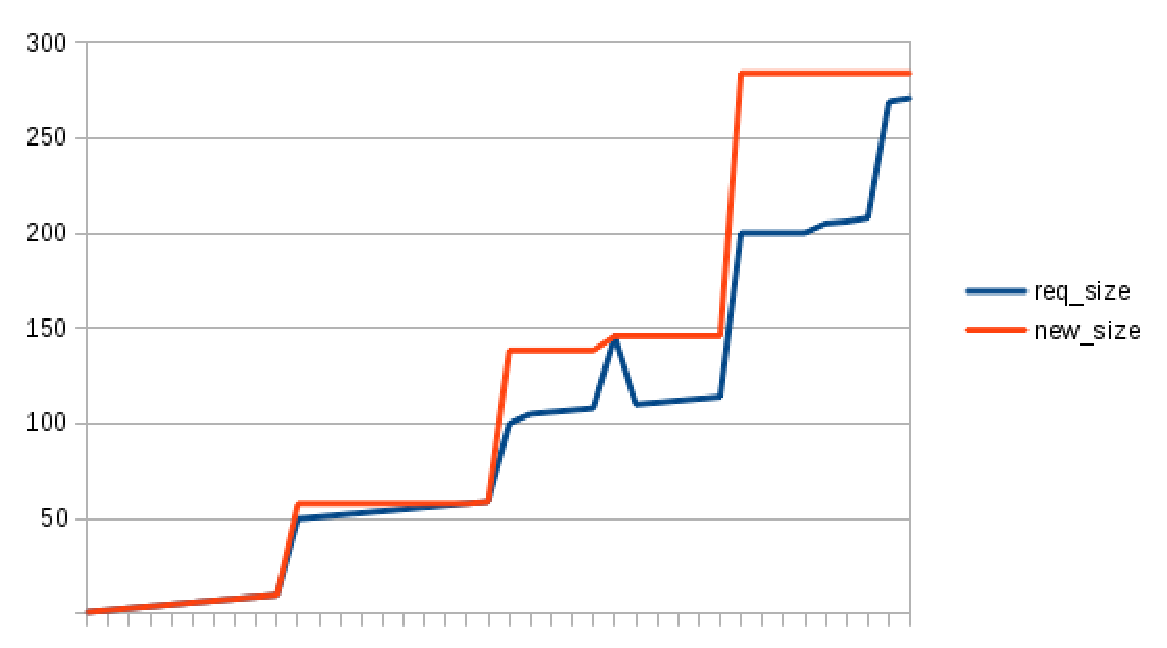
\includegraphics[width=10cm]{pics/realloc}
  \caption{New realloc method.}
  \label{figure:realloc}
\end{figure}